\documentclass[letter]{article}
\usepackage[utf8]{inputenc}
\usepackage[spanish]{babel}

\usepackage{tikz}
\usetikzlibrary{shapes.geometric, arrows}
\graphicspath{ {images/} }
\usepackage{wrapfig}

%%importante ponerlo para tener español

\title{Practica1}
\author{
Rubalcava Cortés Javier Roberto
\and 
Muñoz Carpio Erick David
}
\date{\today}

\usepackage{biblatex}
\addbibresource{references.bib}
\usepackage{graphicx}
%%%sfdasfasffsf
\tikzstyle{startstop} = [rectangle, rounded corners, minimum width=3cm, minimum height=1cm,text centered, draw=black, fill=red!30]

%%\tikzstyle{io} = [trapezium, trapezium left angle=70, trapezium right angle=110, minimum width=3cm, minimum height=1cm, text centered, draw=black, fill=blue!30]
%%la comento por que de momento no la estamos usando
\tikzstyle{process} = [rectangle, minimum width=3cm, minimum height=1cm, text centered, draw=black, fill=orange!30]

\tikzstyle{arrow} = [thick,->,>=stealth]
\begin{document}

\maketitle
\begin{center}
	\textbf{Grupo:602}
\end{center}

\newpage

 
\tableofcontents{}
\newpage



\section{Objetivos.}

\begin{itemize}
	\item Efectuaras alguna recciones quimicas.
	\item Escribirás las ecuaciones completas de las reacciones que efectuaras y las
\end{itemize}

\section{Investigación previa.}
\subsection{Azufre.}
\begin{wrapfigure}{l}{0.25\textwidth}
	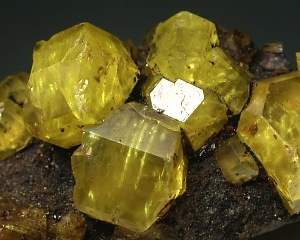
\includegraphics[width=1\linewidth]{azufre} 
	\caption{Axufre en forma de cristal}
	\label{fig:subim1}
\end{wrapfigure}
El azufre es el elemento numero 16 de la tabla periodica, ubicado en la X familia y en el Y grupo. Tiene una masa atomica de 32.065, ademas de tener propiedades electricas de aislante y una resistencia de Z.\par
Se encuentra naturalmente en volcanes, cerca de aguas termales y meteoritos \par
Algunos de los usos que tiene el Azufre es como fertilizante \cite{acuna1991fertilizacion}, la mayoria del azufre se convierte en ácido sulfúrico, el cual se utiliza en refinerias de petróleo, plaguicidas  ,tratamiento de aguas reciduales, baterias de plomo, eliminación de óxido de hierro, fabricacíon de nylon y producción de ácido clorhídrico. \par
%% solucionar el problema de las citas
Lorem ipsum dolor sit amet, consectetur adipiscing elit. Duis id sem libero. Proin vitae purus rutrum, scelerisque turpis non, aliquam massa. Pellentesque vel cursus diam. Curabitur quis ligula nec enim sodales hendrerit. Donec sed risus ipsum. Aenean molestie aliquam nisi, eu eleifend velit bibendum non. Aenean venenatis ligula facilisis, pellentesque metus a, placerat orci. Morbi nec nibh eget turpis viverra mattis quis vel leo. Nunc et ligula sollicitudin, consectetur arcu sed, cursus nisl. Fusce congue porta lorem quis fermentum. Fusce congue eu justo sit amet facilisis.\par
\subsection{Acido sulfhídrico.}
Lorem ipsum dolor sit amet, consectetur adipiscing elit. Duis id sem libero. Proin vitae purus rutrum, scelerisque turpis non, aliquam massa. Pellentesque vel cursus diam. Curabitur quis ligula nec enim sodales hendrerit. Donec sed risus ipsum. Aenean molestie aliquam nisi, eu eleifend velit bibendum non. Aenean venenatis ligula facilisis, pellentesque metus a, placerat orci. Morbi nec nibh eget turpis viverra mattis quis vel leo. Nunc et ligula sollicitudin, consectetur arcu sed, cursus nisl. Fusce congue porta lorem quis fermentum. Fusce congue eu justo sit amet facilisis.\par
\subsection{Acido clorhídrico.}
Lorem ipsum dolor sit amet, consectetur adipiscing elit. Duis id sem libero. Proin vitae purus rutrum, scelerisque turpis non, aliquam massa. Pellentesque vel cursus diam. Curabitur quis ligula nec enim sodales hendrerit. Donec sed risus ipsum. Aenean molestie aliquam nisi, eu eleifend velit bibendum non. Aenean venenatis ligula facilisis, pellentesque metus a, placerat orci. Morbi nec nibh eget turpis viverra mattis quis vel leo. Nunc et ligula sollicitudin, consectetur arcu sed, cursus nisl. Fusce congue porta lorem quis fermentum. Fusce congue eu justo sit amet facilisis.\par
    


\section{Desarrollo experimental.}
\subsection{Diagrama de flujo.}\par
\begin{center}
	\begin{tikzpicture}[node distance=2cm]
		\node (start) [startstop] {Start};
		\node (pro1) [process, below of=start] {En una hoja de papel dividida \par
		 en dos inserta un poco de \textbf{Hierro} y \textbf{Azufre}};
		 \node (pro2) [process, below of=pro1] {Con el \textbf{agitador de vidrio integra perfectamente el Hierro y el  azufre} };
		 \node (pro3) [process, below of=pro2] {Dividir el contenido del papel en dos porciones iguales\textbf{A y B} };
		 \node (pro4) [process, below of=pro3] {inserta el contenido de \textbf{A} en un tubo de ensayo y agrega a este \textbf{ HCL} };
		 \node (pro5) [process, below of=pro4] { inserta el contenido de \textbf{b} en otro tubo de ensayo};
		 \node (pro6) [process, below of=pro5] {Llena el vaso de precipitado con agua hasta la \textbf{mitad} };
		 \node (pro7) [process, below of=pro6] { calienta el tubo de ensayo que contiene la parte \textbf{B} hasta el \textbf{rojo vivo}};
		 \node (pro8) [process, below of=pro7] { Insertar el tubo \textbf{caliente} dentro del vaso con agua fria};
		 
		 \draw [arrow] (start) -- (pro1);
		 \draw [arrow] (pro1) -- (pro2)
		 \draw [arrow] (pro2) -- (pro3);
		 \draw [arrow] (pro3) -- (pro4);
		 \draw [arrow] (pro4) -- (pro5);
		 \draw [arrow] (pro5) -- (pro6);
		 \draw [arrow] (pro6) -- (pro7);
		  \draw [arrow] (pro7) -- (pro8);
		\end{tikzpicture}

\end{center}
\section{Precentación de resultados}
\paragraph{resultado de paso 1}
El hierro tiene un color café y de asemeja al café en polvo y no tiene olor(aparente), el Azufre tiene un color verde limón sin olor(aparente).
\paragraph{resultado del paso 2}
Los elementos mantienen sus propiedades por lo que se le considera mezcla(entre ella el color) como se puede ver en la figura \ref{fig:obs1}
\paragraph{resultado del paso3}
El hierro mantiene sus propiedades magnéticas por lo que fue una mezcla y no un compuesto
+ "los colores de mezclaron un poco pero se seguía separando el hierro del azufre al pasar el imán” como se puede apreciar en \ref{fig:obs2}
\paragraph{resultado del paso4}

\paragraph{resultado del paso5}
 El ácido pasó a tener un color verde-amarrillento y una parte se sedimento 
La temperatura aumento, se libero un gas de un olor un poco desagradable
\paragraph{resultado del paso6}
La mezcla de ácido clorhídrico con el sólido que se formó previamente empezó a burbujear y el olor que salía del tubo de ensayo era parecido al huevo podrido además de que el aviso se volvió de un color gris oscuro a negro
%% a partir de aqui empiezan las imagenes de lo que se observo en la practica, para agregar una imagen se sigue este formato
%%\begin{figure}	
%%	\centering	
%%	\includegraphics[width=0.5\textwidth]{nombre de figura}
%%	\caption{descripcion de figura .}
%%	\label{referencia}
%%\end{figure}

	
\begin{figure}
		
	\centering	
	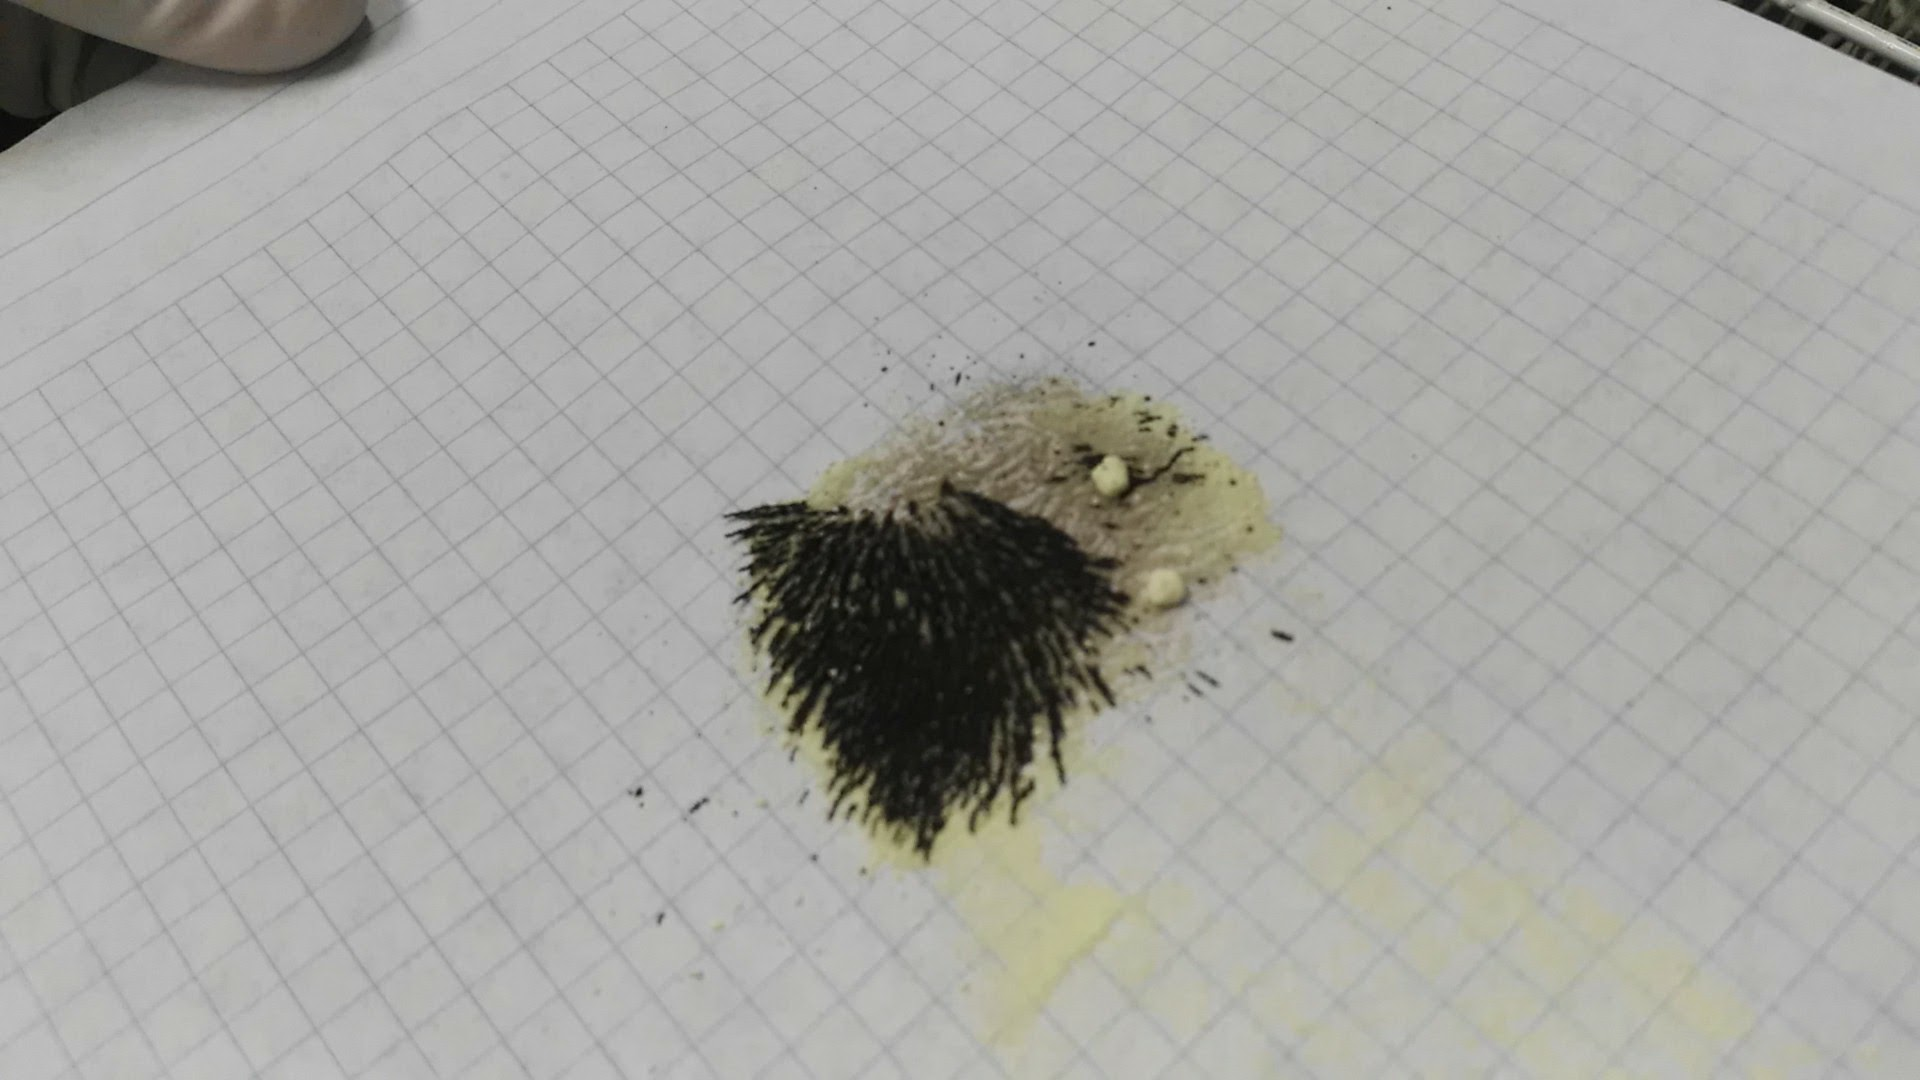
\includegraphics[width=0.5\textwidth]{obs1}
	\caption{La mezcla del hierro con el Azufre.}
	\label{fig:obs1}
\end{figure}
\begin{figure}
	\centering	
	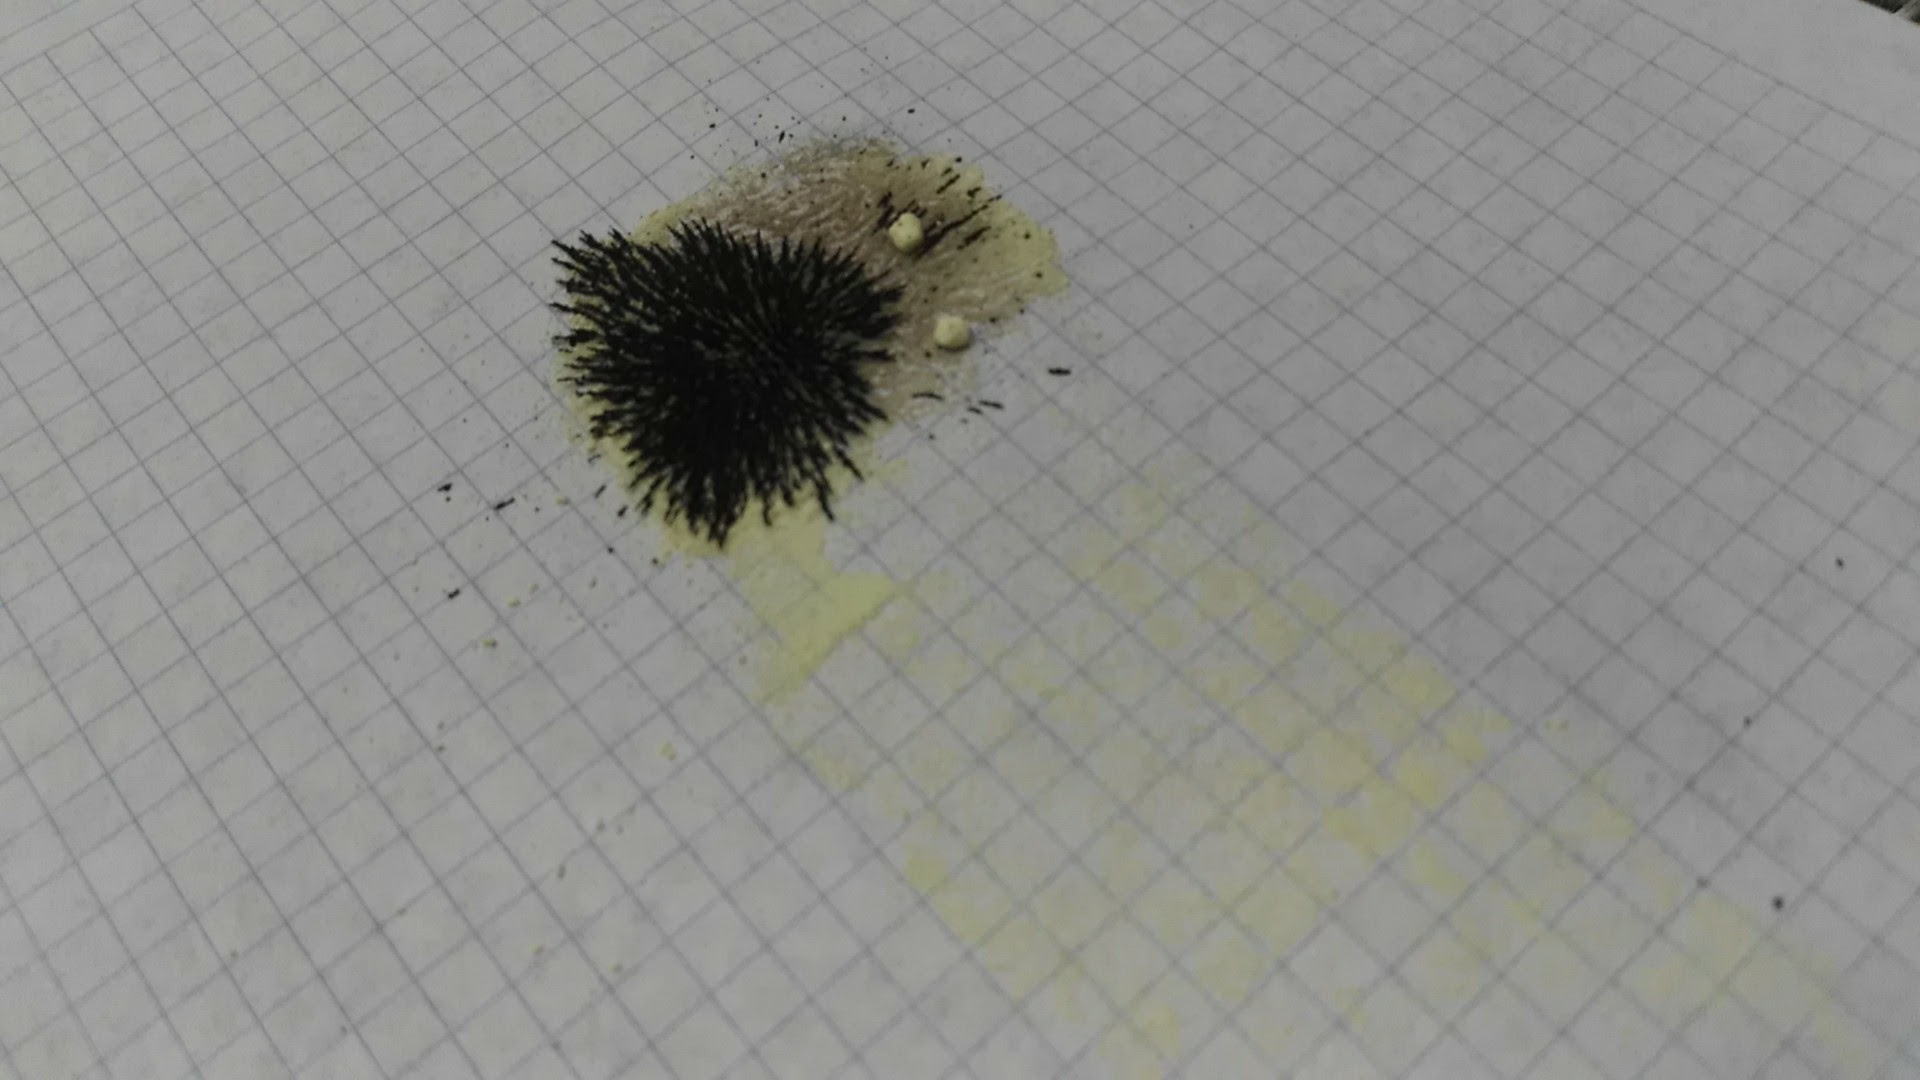
\includegraphics[width=0.5\textwidth]{obs2}
	\caption{La mezcla del hierro con el Azufre reccionan ante el iman.}
	\label{fig:obs2}
\end{figure}

\section{Analisis de resultados.}
Lorem ipsum dolor sit amet, consectetur adipiscing elit. Duis id sem libero. Proin vitae purus rutrum, scelerisque turpis non, aliquam massa. Pellentesque vel cursus diam. Curabitur quis ligula nec enim sodales hendrerit. Donec sed risus ipsum. Aenean molestie aliquam nisi, eu eleifend velit bibendum non. Aenean venenatis ligula facilisis, pellentesque metus a, placerat orci. Morbi nec nibh eget turpis viverra mattis quis vel leo. Nunc et ligula sollicitudin, consectetur arcu sed, cursus nisl. Fusce congue porta lorem quis fermentum. Fusce congue eu justo sit amet facilisis.\par
Lorem ipsum dolor sit amet, consectetur adipiscing elit. Duis id sem libero. Proin vitae purus rutrum, scelerisque turpis non, aliquam massa. Pellentesque vel cursus diam. Curabitur quis ligula nec enim sodales hendrerit. Donec sed risus ipsum. Aenean molestie aliquam nisi, eu eleifend velit bibendum non. Aenean venenatis ligula facilisis, pellentesque metus a, placerat orci. Morbi nec nibh eget turpis viverra mattis quis vel leo. Nunc et ligula sollicitudin, consectetur arcu sed, cursus nisl. Fusce congue porta lorem quis fermentum. Fusce congue eu justo sit amet facilisis.\par


\printbibliography
\end{document}
